\documentclass[dissertation.tex]{subfiles} 
\begin{document}

\chapter{The Compact Muon Solenoid Experiment}
\label{chap:The Compact Muon Solenoid Experiment}
%see detector paper
%overview, pointing out CMS on the ring, coordinate system and theta, eta, phi, rho, ET, pT, pseudorapidity, etc. definition
%picture of the cross-section

The Compact Muon Solenoid (CMS) detector sits at point 5 of the LHC ring, diametrically opposite the ATLAS detector at point 1.  It is a 4$\pi$ hermetic general purpose detector, meaning that it has the capability to detect charged and neutral hadrons, photons, electrons, muons, taus, neutrinos, and non-Standard-Model particles predicted to escape the detector with good efficiency over a large range of rapidity.  Its main distinguishing feature is a superconducting solenoid that provides a 3.8T magnetic field parallel to the beam line.  This strong magnetic field allows precise determination of the momentum and charge of muons and electrons up to a momentum of $\sim$1 TeV.

%explain the CMS coordinate system here

The CMS sub-detectors are arranged in concentric cylindrical layers, plus ``endcaps," around the beam line, as shown in Figure~\ref{fig:CMS_cutaway}.  Closest to the beam line are three layers of silicon pixel detectors, with the innermost at radius 4.4 cm and outermost at radius 10.2 cm \cite{CMS_detector_paper}.  Including the pixel endcaps, the total pixel coverage extends to $\eta$ = 2.5 \cite{CMS_detector_paper}.  The pixel detector plays in important role in determining the proton-proton interaction position (\textit{beam spot}) and the impact parameters of charged particle trajectories, and is critical for the measurement of decay positions some distance from the beam spot (\textit{displaced vertices}), such as those due to the showering and hadronization of a $b$ quark.

The 10 next layers of CMS are comprised of silicon microstrip detectors, with the outermost layer at a radius of 1.3 m from the beam line \cite{CMS_detector_paper}.  As for the pixel detectors, the silicon strip endcaps extecnd tracking coverage to $\eta$ = 2.5.  The silicon microstrip layers are the workhorse of the CMS tracking system, and provide excellent charged particle momentum resolution and track finding efficiency.

Outside the tracking detectors are the calorimeters, starting with the single-layer lead tungstate crystal electromagnetic calorimeter at a radius of 1.3 m from the beam line (location of crystal front faces) \cite{CMS_detector_paper}.  Each crystal is 23 cm long, corresponding to 25.8 radiation lengths ($\mbox{X}_{0}$).  The crystal dimensions are such that most of one electromagnetic shower, and no more, can be contained in a single crystal, leading to excellent energy resolution for photons and electrons.  The electromagnetic calorimeter radial and endcap layers cover a pseudorapidity range up to 3.0.  A lead/silicon sampling calorimeter sits in front of the crystal endcaps to provide better rejection of neutral pions.

The last layer of calorimetry inside the solenoid is the brass/scintillator sampling hadronic calorimeter, which has a radial extent from 1.77-2.95 m \cite{CMS_detector_paper}.

\begin{figure}
	\centering
	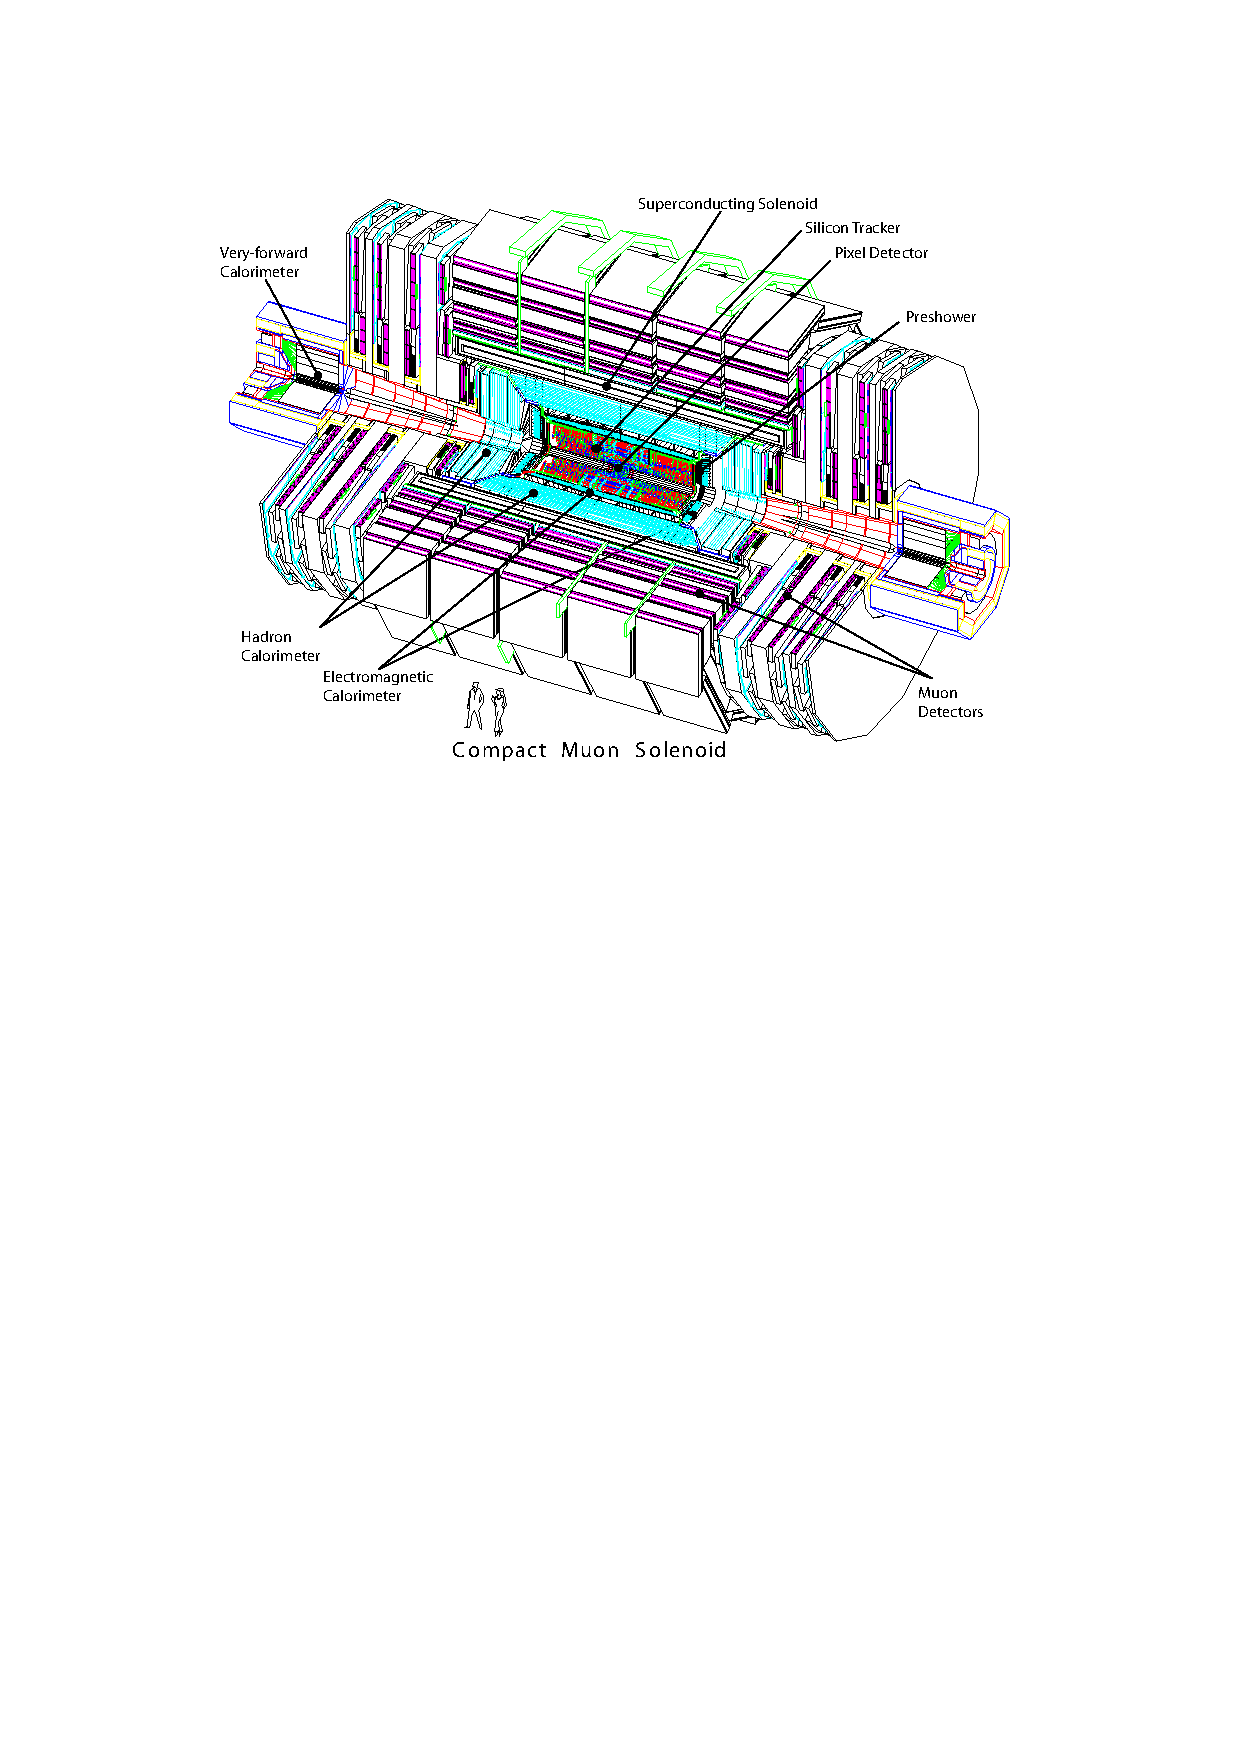
\includegraphics[scale=1.0]{CMS_cutaway}
	\caption{Cutaway view of CMS.  Reprinted from Fig. 1.1 of ref. \cite{CMS_detector_paper}.}
	\label{fig:CMS_cutaway}
\end{figure}

For a thorough description of CMS, see ref. \cite{CMS_detector_paper}, from which much of the information in the section was culled.

\section{The Detectors and Their Operating Principles}
\subsection{Tracking System}
\subsubsection{Pixel Detector}
\subsubsection{Silicon Strip Tracker}
\subsection{Electromagnetic Calorimeter}
\label{sec:Electromagnetic Calorimeter}
%make this big, include EE work
%discuss crystal radiation damage
\subsection{Hadronic Calorimeter}
\subsection{Muon System}
%spend very little time on this
\subsection{Far Forward Calorimetry}
%spend very little time on this

\section{Triggering, Data Acquisition, and Data Transfer}
\subsection{Level 1 and High Level Trigger Systems}
\label{sec:Level 1 and High Level Trigger Systems}
%talk about trigger primitives for the ECAL especially (there is a reference to this section from the HLT section in ch. 6 when we talk about L1 seeds), SR, etc.
\subsection{Data Acquisition System}
\subsection{Data Processing and Transfer to Computing Centers}
\label{sec:Data Processing and Transfer to Computing Centers}
%define lumi section

Lorum ipsum fuck Republicans.

\end{document}